\documentclass{article}
\usepackage{hyperref}
	\hypersetup{
	    colorlinks,
	    linkcolor={red!50!black},
	    citecolor={blue!50!black},
	    urlcolor={blue!80!black}
	}
%%%%%%%%%%%%%% Packages used for drawing the trees %%%%%%%%%%%%%%%%%%%%%%%%%
\usepackage{graphicx}

% for coloring figures; load before tikz to use dvipsnames
% if you get option clash for xcolor, replace 'Green' with 'cyan' in color defs
\usepackage{xcolor}
%\usepackage{tikz} % for drawing (GT graphs in particular)
\usepackage{forest} % should be better than the standard tikz trees
	\usetikzlibrary{shapes} % for triangle shaped nodes
	\usetikzlibrary{calc} % for calculating coordinates
\usepackage{xparse}	% for defining macros with optional argumentss

%%%%%%%%%%%%%%% Node style definitions %%%%%%%%%%%%%%%%%%%%%%%%%%%%%%%%%%%%%%%%%%%%%%
% node sizes setup
\newlength{\nodesize}
% this is meant to be adjustable, but doing so messes up level distances, and requires adjusting l sep for chance and terminal nodes
\setlength{\nodesize}{2.5em}
% Player colors
\colorlet{chance_color}{black}
\colorlet{pl0_color}{chance_color}
\colorlet{chance_text}{white}
\colorlet{pl1_color}{magenta!50}
\colorlet{pl2_color}{cyan!50}
\colorlet{pl0_infoset_color}{pl0_color}
\colorlet{pl1_infoset_color}{magenta!75}
\colorlet{pl2_infoset_color}{cyan!75}
% player 1 and 2, chance, terminal nodes
\forestset{
	basenode/.style = {draw,
		inner sep = 0,
		outer ysep = 0,
		minimum size = \nodesize,
		anchor = north
	},
	playernode/.style={basenode, 
		shape = regular polygon,
		regular polygon sides = 3,
	},
	pl1/.style={playernode, fill=pl1_color},
	pl2/.style={playernode, fill=pl2_color, shape border rotate=180},
	chance/.style = {basenode,
		fill=pl0_color, text=chance_text,
		circle,
		minimum size=0.75*\nodesize,
%		child anchor=center,
		l sep=0.4765\nodesize,
	},
	terminal/.style = {basenode,
		shape = regular polygon,
		regular polygon sides = 4,
		l sep=0.47\nodesize,
		minimum size = 1.07\nodesize
	}
}
% information sets
\tikzset{
	partition/.style = {
		draw,
%		inner xsep = 0.1\nodesize,
%		inner ysep = 0.1\nodesize,
		rounded corners = 5,
		inner sep=0.1\nodesize,
	},
	infoset/.style = {
		partition,
		draw=pl1_infoset_color,
	},
	augmented/.style = {
		dashed
	},
	opponent/.style = {
		draw=pl2_infoset_color,
		% bigger separation than pl1, to prevent overlapping with pl1 infosets
		inner sep=0.225\nodesize,
	},
	% triangles are not symmetric, the ``classical'' infosets shift the rectangles
	% to make the spaces above and below nodes look more similar
	pl1_cl_infoset/.style = {infoset, yshift=-0.035\nodesize},
	pl2_cl_infoset/.style = {infoset,
		opponent,
		inner sep=0.1\nodesize,
		yshift=0.035\nodesize
	},
	public_state/.style = {
		partition,
		draw=pl0_infoset_color,
		inner sep=0.125\nodesize,
		rounded corners = 7,
	},
}
% infosets connected by lines
\tikzset{
	line_infoset/.style = {
		draw=pl1_infoset_color,
		dashed
	},
	opp_line_infoset/.style = {
		draw=pl2_infoset_color,
		dashed
	}
}
% a shortcut for listing all corners of a triangle-node
\newcommand{\corners}[1]{#1.corner 1)(#1.corner 2)(#1.corner 3}
% measure the angle between node A and B (without '()' brackets around)
% and save it into `\angle`
\newcommand{\measureAngle}[2]{
	\node(dummy#1)[draw=none] at (#1) {};
	\node(dummy#2)[draw=none] at (#2) {};
	\pgfmathanglebetweenpoints
		{\pgfpointanchor{dummy#1}{center}}
		{\pgfpointanchor{dummy#2}{center}}
	\edef\angle{\pgfmathresult}
}
%%%%%%%%%%%%%%%%%%%%%%%%%%%%%%%
%%%%%%%%% just some nonsense to be able to have infosets in the background
\pgfdeclarelayer{bg}    % declare background layer
\pgfsetlayers{bg,main}  % set the order of the layers (main is the standard layer)
%%%%%%%%%%%%%%%%%%%%%%%%%%%%%%%%%

\begin{document}

\title{Drawing game theory trees using \texttt{FOREST}}
\author{Vojta Kovarik}
\maketitle


To use these styles, use \textbackslash input\{GT\_trees\} -- it imports all the necessary packages.
This document provides examples of drawing pictures in TikZ + Forest, using some macros and styles that I have defined.
Recommended order of reading is: if you only need one or two examples, and don't need to fine-tune them, then just copy the code from an example that you like.
If you need more details, something doesn't behave as expected, or you start encountering errors, then read the section about TikZ/Forest basics, and the section relevant to your problem.

If this text doesn't solve your problem, consult the \href{http://www.chiark.greenend.org.uk/doc/texlive-doc/latex/forest/forest.pdf}{forest documentation} and \href{https://sourceforge.net/projects/pgf/}{PGF/TikZ documentation} (or draw your picture using some other tool).
For drawing game trees without colored and/or triangle shaped player nodes, see \href{http://www.sfu.ca/~haiyunc/notes/Game_Trees_with_TikZ.pdf}{Drawing Game Trees with Ti$k$Z}.

\begin{figure}[h]
\centering
\begin{forest}
[, chance, l sep+=0.3\nodesize, s sep+=0.05\nodesize, 
	[,pl2, edge label={node[midway,sloped,above]{left}}
		[,pl1, [0] ]
		[,pl1, [1] ]
	]
	[,pl2, edge label={node[midway,sloped,above]{right}}
		[,pl1, [1] ]
		[,pl1, [0] ]
	]
]
\node [pl2_cl_infoset, fit=(\corners{!1})(\corners{!2})] {};
\node [pl1_cl_infoset, fit=(\corners{!11})(\corners{!12})] {I};
\node [pl1_cl_infoset, fit=(\corners{!21})(\corners{!22})] {J};
\end{forest}
\caption{The purpose of this document is to allow a simple creation of game trees, such as this one, without having to learn the whole Ti$k$Z package.}
\label{fig:example}
\end{figure}


\tableofcontents



\section{Basic constructions using TikZ and Forest}

\subsection{Forest syntax}
The basic syntax using forest is just square brackets, commas serve to separate arguments but do not throw errors when there are too many of them. It is not sensitive to spaces, tabs and line ends. However, \emph{empty lines throw errors}.  See the latex code for examples.

\begin{forest}
[
	[]
	[
		[] [] []	
	]
	[
		[] [] 	
	]
]
\end{forest}
\begin{forest}
[[][[][][]][[][]]]
\end{forest}
\begin{forest}
[ [], [ [][][] ], [ [][] ] ]
\end{forest}
\begin{forest}
[,,,,,,,
	[,,,,,,,,,]
	[,,,,
		[,,,],,, [,,] [,,,],,,,
	],,,
	[,,,
		[,,,],,, [,,] 	,,
	],,,
]
\end{forest}
\begin{forest}
% uncommenting the empty line throws an error
[
%
	[]
	[
		[] [] []	
	]
	[
		[] [] 	
	]
]
\end{forest}

\subsection{Formatting nodes}

The first (optional) argument in each node is the text, other arguments influence formatting, and can be used in any order.

\begin{forest}
[root
	[1,draw,circle]
	[2,draw,rectangle
		[{$\sqrt[4]{3}$}] [text opacity,text opacity=0.5]	
	]
	[,phantom
		[phantom\\parent,align=center]	
	]
	[3,draw,fill=blue,regular polygon, regular polygon sides=7, text=white
		[red node,red] [red]
	]
]
\end{forest}

\subsection{Formatting multiple nodes at once}

Multiple nodes can be formatted at the same time with the help of the `for tree/children/descendants' syntax:

\begin{forest}
[0[1,red [2], [3 [4][5][6] ], [7 [8][9] ] ]]
\end{forest}
\begin{forest}
[0[1,for tree={red} [2], [3 [4][5][6] ], [7 [8][9] ] ]]
\end{forest}
\begin{forest}
[0[1,for descendants={red} [2], [3 [4][5][6] ], [7 [8][9] ] ]]
\end{forest}
\begin{forest}
[0[1,for children={red} [2], [3 [4][5][6] ], [7 [8][9] ] ]]
\end{forest}

\subsection{Changing the tree geometry}

The position of a node/nodes can be adjusted using `l', `xshift', `yshift' and `s sep' (and in many other ways). Growth direction can be adjusted using `grow` argument (which takes either numeric angles or directions such as `south east').

\begin{forest}
[1 [2] [3[4][5][6]] [7[8][9]] ]
\end{forest}
\begin{forest}
[1 [2] [3,xshift=0.25cm,yshift=-0.5cm[4][5][6]] [7[8][9]] ]
\end{forest}
\begin{forest}
for tree={grow=north east}
[1 [2] [3[4][5][6]] [7[8][9]] ]
\end{forest}

\begin{forest}
for tree={s sep+=2em}
[1 [2] [3[4][5][6]] [7[8][9]] ]
\end{forest}
\begin{forest}
[1 [2] [3,s sep+=2em[4][5][6]] [7,s sep-=1em[8][9]] ]
\end{forest}
\begin{forest}
for tree={l+=10pt}
[1 [2] [3[4][5][6]] [7[8][9]] ]
\end{forest}

Use `tier` enforce that specific nodes are vertically aligned:

\begin{forest}
[1
	[2, ]
	[3 [4] [5] [6] ]
]
\end{forest}
\begin{forest}
[1
	[2,tier=customThingy]
	[3 [4,tier=customThingy][5][6] ]
]
\end{forest}



\section{Custom game theory constructions}

\subsection{Node styles}

The predefined game-theory nodes styles are `pl1', `pl2', `chance' and `terminal' (which can be ignored if you don't like it):

\begin{forest}
[, pl1,
	[, pl2,
	% if you forget the comma, it won't work :P
%		[,pl1] [,pl1] [pl1]	
		[,pl1] [,pl1 [$\frac{1}{3}$,terminal]] [,pl1 [1,terminal] [z,terminal] ]	
	]
	[, pl2, for descendants={chance},
		[] [] []
	]
	[, pl2,
		[,chance] [,pl1 [1] [0.5]] [,pl2] [,pl1]
	]
]
\end{forest}

Minimizer and maximizer nodes might end up too close to each other. If you don't want that, you have to adjust them manually (the picture is an overkill):

\begin{forest}
[, pl2,
	[,pl1]
	[,pl1]
	[,pl1]
	[,pl2]
]
\end{forest}
\begin{forest}
[, pl2, xshift=1cm,
	[,pl1]
	[,pl1]
	[,pl1]
	[,pl2,xshift=2cm]
]
\end{forest}

\subsection{Information sets}

We show two ways of drawing information sets -- rectangles and connecting by dashed lines.

\subsubsection{Partitioning by rectangles}

You can name nodes (and other objects) and create information sets using the ``\textbackslash node [style, fit=(nodeA)(nodeB)] {};'' syntax.
For triangle nodes, use (\textbackslash corner\{nodeA\}) instead of (nodeA).
The predefined styles are `infoset', `opponent' and `augmented'. Alternatively you can use `cl\_infoset' and `cl\_opp\_infoset' to draw classical information sets which are better aligned with the corresponding triangles (but not with each other, if they appear on the same line).

\begin{forest}
[, phantom, s sep+=0.65\nodesize,
	[1,pl1,name=1]
	[2,pl1,name=2]
	[3,pl1,name=3]
	[4,pl1,name=4]
	[5,pl1,name=5
		[A,chance,name=5A]
		[B,pl1,name=5B]
	]
	[6,pl1,name=6]
	[7,pl2,name=7]	
	[8,chance,name=8]
]
\node [pl1_cl_infoset, fit=(\corners{1})(\corners{2})] {};
\node [infoset, fit=(\corners{3})(\corners{4})] {};
\node [infoset, opponent, augmented, fit=(\corners{5})(5A)(\corners{5B})] {};
\node [public_state, fit=(\corners{6})(8)] {};
\end{forest}

\begin{forest}
[, phantom, s sep+=0.8\nodesize,
	[1,pl1,name=1]
	[2,pl1,name=2]
	[3,pl1,name=3]
	[4,pl1,name=4]
	[5,pl1,name=5
		[A,chance,name=5A]
		[B,pl1,name=5B]
	]
	[6,pl1,name=6]
	[7,pl2,name=7]	
	[8,chance,name=8]
]
\node(InfosetName1) [pl1_cl_infoset, fit=(\corners{1})(\corners{2})] {I1};
\node(InfosetName2) [infoset, fit=(\corners{3})(\corners{4})] {I2};
\node(J1) [infoset, opponent, augmented,
		fit=(\corners{5})(5A)(\corners{5B}),
		label=south east:{J}] {};
\node(J2) [pl2_cl_infoset, fit=(\corners{7})] {};
\node [public_state, fit=(\corners{6})(8)(J2), label=below:{public state $S$}] {};
\node [public_state, fit=(InfosetName1)(InfosetName2), label={$T$}] {};
\end{forest}

For infosets containing stuff from different levels, you can also use rotated infosets by adding `rotate fit=$\alpha$', where $\alpha$ is the rotation angle. The `\textbackslash measureAngle' macro measures the angle automatically and saves it into `\textbackslash angle'.

\begin{forest}
[5,pl1,name=5,s sep+=1.5\nodesize
	[A,chance,name=5A]
	[B,pl1,name=5B]
]
%
\measureAngle{5}{5B}
\node [infoset, rotate fit=\angle, fit=(\corners{5})(\corners{5B})] {};
%
\measureAngle{5}{5A}
\node [infoset, opponent, augmented, rotate fit=\angle, fit=(\corners{5})(5A)] {};
\end{forest}

\subsubsection{Connecting by dashed lines}

You can also indicate infosets using curved dashed lines, using the `\textbackslash draw[line\_infoset, bend left/right ] (nodeA) to (nodeB)' syntax. For player 2 color, use `opp\_line\_infoset'.

\begin{forest}
[, chance
	[,pl1]
	[,pl1]
	[,pl2]
	[,pl2]
]
\begin{pgfonlayer}{bg}    % select the background layer
	\draw[line_infoset, bend left] (!1) to (!2);
	\draw[opp_line_infoset, bend right] (!3) to (!4);
\end{pgfonlayer}
\end{forest}

You can also specify the exact angle, and where should the lines start and end:

\begin{forest}
[, chance
	[,pl1]
	[,pl1]
	[,pl2]
	[,pl2]
]
\begin{pgfonlayer}{bg}    % select the background layer
	\draw[line_infoset, bend right] (!3.south) to (!4.corner 3);
		\draw[line_infoset, augmented, bend left] (!3.north) to (!4.north);
	\draw[opp_line_infoset, out=90, in = 135] (!1) to (!2);
\end{pgfonlayer}
\end{forest}

\subsection{Multiple partitions in a single picture}

When multiple partitions are present in a single picture, you might have to increase the distances between nodes. This increases the size of the picture a lot, and there might often be a better solution (only drawing one player, drawing each player in a separate picture, drawing one player's infosets with dashed lines).


Adding infosets for different players (there should be a better solution than putting it all into a single picture -- this is just for illustration):

%%%%%%%%%%%%%%%%%%%%%%%%%%%%%%%%%%%%%%%%%%%%%%%%%%%%%%%%%%%%%%%%%%%%%%%%%%%%%%%%%%%%
Basic example with no information sets, with commented-out lines for increasing the size between nodes:

\begin{forest}
% uncomment of the following lines to increase distances between nodes
% depending on how many information partitions appear in the picture
% to keep the tree more compact, only add it to specific nodes
%for tree={l+=0}, for tree={s sep+=0},							% histories only
%for tree={l+=0}, for tree={s sep+=0.2\nodesize},				% only 1 type of partition
%for tree={l+=0.3\nodesize}, for tree={s sep+=0.5\nodesize},	% 2 types of partition
%for tree={l+=0.6\nodesize}, for tree={s sep+=0.8\nodesize},	% 3 types of partition
%
[, pl1, name=R,
	% increase gaps between maximizer and minimizer siblings and re-align the parents
	xshift=0.25\nodesize, !3.xshift=0.5\nodesize, !33.xshift=1\nodesize,
	[, pl2, name=A, for descendants={pl1},
		[] [] []	
	]
	[, pl1, name=B , for descendants={chance},
		[] [] []
	]
	[, chance, name=C,
		[,pl2] [,pl2] [,pl1]
	]
]
\end{forest}
%%%%%%%%%%%%%%%%%%%%%%%%%%%%%%%%%%%%%%%%%%%%%%%%%%%%%%%%%%%%%%%%%%%%%%%%%%%%%%%%%%%%

%%%%%%%%%%%%%%%%%%%%%%%%%%%%%%%%%%%%%%%%%%%%%%%%%%%%%%%%%%%%%%%%%%%%%%%%%%%%%%%%%%%%
Maximizer's classical and augmented information sets.

\begin{forest}
for tree={l+=0}, for tree={s sep+=0.2\nodesize},				% only 1 type of partition
[, pl1, name=R,
	!33.xshift=1.25\nodesize,
	[, pl2, name=A, for descendants={pl1},
		[] [] []	
	]
	[, pl1, name=B, for descendants={chance},
		[] [] []
	]
	[, chance, name=C,
		[,pl2] [,pl2] [,pl1]
	]
]
\node(I1) [infoset, fit=(\corners{R})] {};
\node(I2) [infoset, fit=(\corners{B})] {};
\node(I3) [infoset, fit=(\corners{A!1})(\corners{A!3})] {};
\node(I4) [infoset, fit=(\corners{C!3})] {};
\node(I5) [infoset, augmented, fit=(\corners{A}) ] {};
\node(I6) [infoset, augmented, fit=(C)] {};
\node(I7) [infoset, augmented, fit=(B!1)] {};
\node(I8) [infoset, augmented, fit=(B!2)] {};
\node(I9) [infoset, augmented, fit=(B!3)] {};
\node(I10) [infoset, augmented, fit=(\corners{C!1}) (\corners{C!2}) ] {};
\end{forest}
%%%%%%%%%%%%%%%%%%%%%%%%%%%%%%%%%%%%%%%%%%%%%%%%%%%%%%%%%%%%%%%%%%%%%%%%%%%%%%%%%%%%

\vspace{4mm}
%%%%%%%%%%%%%%%%%%%%%%%%%%%%%%%%%%%%%%%%%%%%%%%%%%%%%%%%%%%%%%%%%%%%%%%%%%%%%%%%%%%%
Infosets of both players.

\begin{forest}
for tree={l+=0.3\nodesize}, for tree={s sep+=0.5\nodesize},	% 2 types of partition
[, pl1, name=R,
	!33.xshift=1.5\nodesize,
	[, pl2, name=A, for descendants={pl1},
		[] [] []	
	]
	[, pl1, name=B, for descendants={chance},
		[] [] []
	]
	[, chance, name=C,
		[,pl2] [,pl2] [,pl1]
	]
]
\node(I1) [infoset, fit=(\corners{R})] {};
\node(I2) [infoset, fit=(\corners{B})] {};
\node(I3) [infoset, fit=(\corners{A!1})(\corners{A!3})] {};
\node(I4) [infoset, fit=(\corners{C!3})] {};
\node(I5) [infoset, augmented, fit=(\corners{A}) ] {};
\node(I6) [infoset, augmented, fit=(C)] {};
\node(I7) [infoset, augmented, fit=(B!1)] {};
\node(I8) [infoset, augmented, fit=(B!2)] {};
\node(I9) [infoset, augmented, fit=(B!3)] {};
\node(I10) [infoset, augmented, fit=(\corners{C!1}) (\corners{C!2}) ] {};
%
\node(J1) [infoset, opponent, augmented, fit=(\corners{R})(\corners{B})(C)] {};
\node(J2) [infoset, opponent, augmented, fit=(B!1)(B!3)] {};
\node(J3) [infoset, opponent, augmented, fit=(\corners{C!3})] {};
\node(J4) [infoset, opponent, augmented, fit=(\corners{A!1}) ] {};
\node(J5) [infoset, opponent, augmented, fit=(\corners{A!2}) ] {};
\node(J6) [infoset, opponent, augmented, fit=(\corners{A!3}) ] {};
\node(J7) [infoset, opponent, fit=(\corners{C!1})(\corners{C!2}) ] {};
\node(J8) [infoset, opponent, fit=(\corners{A})] {};
\end{forest}
%%%%%%%%%%%%%%%%%%%%%%%%%%%%%%%%%%%%%%%%%%%%%%%%%%%%%%%%%%%%%%%%%%%%%%%%%%%%%%%%%%%%

%%%%%%%%%%%%%%%%%%%%%%%%%%%%%%%%%%%%%%%%%%%%%%%%%%%%%%%%%%%%%%%%%%%%%%%%%%%%%%%%%%%%
The `fit` function can be used not only with nodes as an input, but also with information sets -- this is useful when creating public states.

\begin{forest}
for tree={s sep+=0.8\nodesize},	% 3 types of partition
[, pl1, name=R, for descendants={l+=0.6\nodesize},
	!33.xshift=1.75\nodesize,
	[, pl2, name=A, for descendants={pl1},
		[] [] []	
	]
	[, pl1, name=B, for descendants={chance},
		[] [] []
	]
	[, chance, name=C,
		[,pl2] [,pl2] [,pl1]
	]
]
\node(I1) [infoset, fit=(\corners{R})] {};
\node(I2) [infoset, fit=(\corners{B})] {};
\node(I3) [infoset, fit=(\corners{A!1})(\corners{A!3})] {};
\node(I4) [infoset, fit=(\corners{C!3})] {};
\node(I5) [infoset, augmented, fit=(\corners{A}) ] {};
\node(I6) [infoset, augmented, fit=(C)] {};
\node(I7) [infoset, augmented, fit=(B!1)] {};
\node(I8) [infoset, augmented, fit=(B!2)] {};
\node(I9) [infoset, augmented, fit=(B!3)] {};
\node(I10) [infoset, augmented, fit=(\corners{C!1}) (\corners{C!2}) ] {};
%
\node(J1) [infoset, opponent, augmented, fit=(\corners{R})(\corners{B})(C)] {};
\node(J2) [infoset, opponent, augmented, fit=(B!1)(B!3)] {};
\node(J3) [infoset, opponent, augmented, fit=(\corners{C!3})] {};
\node(J4) [infoset, opponent, augmented, fit=(\corners{A!1}) ] {};
\node(J5) [infoset, opponent, augmented, fit=(\corners{A!2}) ] {};
\node(J6) [infoset, opponent, augmented, fit=(\corners{A!3}) ] {};
\node(J7) [infoset, opponent, fit=(\corners{C!1})(\corners{C!2}) ] {};
\node(J8) [infoset, opponent, fit=(\corners{A})] {};
%
\node [public_state, fit=(I5)(J8)] {};
\node [public_state, fit=(J4)(J5)(J6)(I3)] {};
\node [public_state, fit=(I1)(I2)(I6)(J1)] {};
\node [public_state, fit=(J2)(I7)(I8)(I9)] {};
\node [public_state, fit=(I1)(I2)(I6)(J1)] {};
\node [public_state, fit=(J7)] {};
\node [public_state, fit=(J3)] {};
\end{forest}
%%%%%%%%%%%%%%%%%%%%%%%%%%%%%%%%%%%%%%%%%%%%%%%%%%%%%%%%%%%%%%%%%%%%%%%%%%%%%%%%%%%%

\vspace{4mm}
%%%%%%%%%%%%%%%%%%%%%%%%%%%%%%%%%%%%%%%%%%%%%%%%%%%%%%%%%%%%%%%%%%%%%%%%%%%%%%%%%%%%
The size can be often further reduced by fine-tuning `s sep', `l' and `l sep' for specific nodes (but it takes time):

\begin{forest}
[, pl1, name=R,
	l sep-=0.4\nodesize,
	s sep+=0.8\nodesize,
	!33.xshift=1.75\nodesize,
	[, pl2, name=A,
		for descendants={pl1},
		for descendants={l+=0.6\nodesize},
		s sep+=0.4\nodesize,
		[] [] []	
	]
	[, pl1, name=B,
		for descendants={chance},
		for descendants={l+=0.6\nodesize},
		s sep+=0.3\nodesize,
		[] [] []
	]
	[, chance, name=C, for descendants={l+=0.6\nodesize},
		[,pl2] [,pl2] [,pl1]
	]
]
\node(I1) [infoset, fit=(\corners{R})] {};
\node(I2) [infoset, fit=(\corners{B})] {};
\node(I3) [infoset, fit=(\corners{A!1})(\corners{A!3})] {};
\node(I4) [infoset, fit=(\corners{C!3})] {};
\node(I5) [infoset, augmented, fit=(\corners{A}) ] {};
\node(I6) [infoset, augmented, fit=(C)] {};
\node(I7) [infoset, augmented, fit=(B!1)] {};
\node(I8) [infoset, augmented, fit=(B!2)] {};
\node(I9) [infoset, augmented, fit=(B!3)] {};
\node(I10) [infoset, augmented, fit=(\corners{C!1}) (\corners{C!2}) ] {};
%
\node(J1) [infoset, opponent, augmented, fit=(\corners{R})(\corners{B})(C)] {};
\node(J2) [infoset, opponent, augmented, fit=(B!1)(B!3)] {};
\node(J3) [infoset, opponent, augmented, fit=(\corners{C!3})] {};
\node(J4) [infoset, opponent, augmented, fit=(\corners{A!1}) ] {};
\node(J5) [infoset, opponent, augmented, fit=(\corners{A!2}) ] {};
\node(J6) [infoset, opponent, augmented, fit=(\corners{A!3}) ] {};
\node(J7) [infoset, opponent, fit=(\corners{C!1})(\corners{C!2}) ] {};
\node(J8) [infoset, opponent, fit=(\corners{A})] {};
%
\node [public_state, fit=(I5)(J8)] {};
\node [public_state, fit=(J4)(J5)(J6)(I3)] {};
\node [public_state, fit=(I1)(I2)(I6)(J1)] {};
\node [public_state, fit=(J2)(I7)(I8)(I9)] {};
\node [public_state, fit=(I1)(I2)(I6)(J1)] {};
\node [public_state, fit=(J7)] {};
\node [public_state, fit=(J3)] {};
\end{forest}
%%%%%%%%%%%%%%%%%%%%%%%%%%%%%%%%%%%%%%%%%%%%%%%%%%%%%%%%%%%%%%%%%%%%%%%%%%%%%%%%%%%%

\section{Putting pictures into other text}

\subsection{Standard figure syntax}
Pictures can be added directly into a specific place by just using the `\textbackslash begin\{forest\} \dots \textbackslash end\{forest\}' syntax.
You can also wrap it in the `figure' environment as usual (Figure~\ref{fig:sample}).

\begin{figure}[h]
\centering
\begin{forest}
[d, pl1 [f,terminal] [l,chance] ]
\end{forest}
\caption{A sample figure. The label goes \emph{after} the caption.}
\label{fig:sample}
\end{figure}

\subsection{Scaling pictures}
%%%%%%%%%%%%%%%% Scaling pictures %%%%%%%%%%%%%%%%%%%%%%%%%%%%%%%%%%%%%%%%%%%%%%%%%%
You can also scale pictures with scalebox:

\begin{forest}
[d, pl1 [f,terminal] [l,chance] ]
\end{forest}
\scalebox{0.5}{
\begin{forest}
[d, pl1 [f,terminal] [l,chance] ]
\end{forest}
}

There should be other ways of scaling the pictures, namely via adjusting the `\textbackslash nodesize' parameter.

% this should work, but it messes up level distances, and requires adjusting l sep for chance and terminal nodes
\begin{forest}
[d, pl1 [f,terminal] [l,chance] ]
\end{forest}
%
\setlength{\nodesize}{1.25em}
\begin{forest}
[d, pl1 [f,terminal] [l,chance] ]
\end{forest}
\setlength{\nodesize}{2.5em}
%
\setlength{\nodesize}{4em}
\begin{forest}
[d, pl1 [f,terminal] [l,chance] ]
\end{forest}
\setlength{\nodesize}{2.5em}

Unfortunately, this doesn't work well with infosets, and would (currently) require adjusting other parameters manually:

\begin{forest}
[d, pl1 [f,terminal] [l,chance] ]
\node [infoset, fit=(\corners{!}) ] {};
\node [infoset, fit=(!1) ] {};
\node [infoset, fit=(!2) ] {};
\end{forest}
%
\setlength{\nodesize}{1.25em}
\begin{forest}
[d, pl1 [f,terminal] [l,chance] ]
\node [infoset, fit=(\corners{!}) ] {};
\node [infoset, fit=(!1) ] {};
\node [infoset, fit=(!2) ] {};
\end{forest}
\setlength{\nodesize}{2.5em}
%
\setlength{\nodesize}{4em}
\begin{forest}
[d, pl1 [f,terminal] [l,chance] ]
\node [infoset, fit=(\corners{!}) ] {};
\node [infoset, fit=(!1) ] {};
\node [infoset, fit=(!2) ] {};
\end{forest}
\setlength{\nodesize}{2.5em}
%
%% this should work, but doesn't atm (\nodesize prevents it from working)
%% optimal way would be setting \nodesize to a multiple of default node size
%\footnotesize{
%\begin{forest}
%[d, pl1 [f,terminal] [l,chance] ]
%\end{forest}
%}
%%%%%%%%%%%%%%%%%%%%%%%%%%%%%%%%%%%%%%%%%%%%%%%%%%%%%%%%%%%%%%%%%%%%%%%%%%%%%%%%%%%%%%%%%%%%



%\begin{forest}
%delay={for tree={grow=east, anchor=mid}}
%[A, pl1[B, pl2 [C, pl1 [D, chance]]]]
%\end{forest}

\section{Naming nodes, infosets, and actions}
\subsection{Labels}
Labels can be specified with the `label=\{[optional arguments] angle : label text\}' syntax. Multi-line labels can be done with the `align=...' environment (see F).

\begin{forest}
[,phantom, s sep+=1\nodesize 
	[A, pl1, label={a) default} ]
	[B, pl1, label=left:{b) left} ]
	[C, pl1, label=north west:{c) NW} ]
	[D, pl1, label={[label distance=.5cm] 120: {d) $\alpha$+dist.} } ]
	[E, pl1, label={[xshift=.25cm]above: {e) x/y shift}} ]
	[F, pl1, label={
				[rotate=30,align=left, label distance = 0.25cm]
				right:{f) rotated\\label}} ]
]
\end{forest}
\subsection{Extra nodes with text via TikZ}
You can also add extra nodes with text manually, using TikZ:

\begin{forest}
[,phantom, s sep+=1\nodesize 
	[, pl1, name=nodeA]
	[B, pl1, name=nodeB]
	[C, pl1, name=nodeC]
]
\node[red] at (nodeA) {label A};
\node[yshift=0.75\nodesize] at (nodeB) {label B};
\node[anchor=west] at ($(nodeC)+(0.4\nodesize,0)$) {label C};
\end{forest}

\subsection{Decorating edges}

Edges can be decorated with normal tikz syntax:

\begin{forest}
[R, chance
	[A, pl1, edge={dashed} ]
	[B, pl1, edge={draw=none} ]
	[C, pl1, edge={red} ]
]
\end{forest}

You can also put labels on top of edges:

\begin{forest}
[R, chance, s sep+=1\nodesize 
	[A, pl1, edge={sloped}, edge label={node[midway,above]{action}} ]
	[B, pl1, edge label={node[pos=1,right]{GAH}} ]
	[C, pl1, edge label={node[sloped,rotate=90,midway,above,anchor=west]{rotated}} ]
]
\end{forest}

%\subsection{Hiding text}
%If you want to hide all text (e.g. when the game has already been described earlier), just set it's opacity to 0. Somehow this messes up positioning, but if all you want to do is create the pdf, then it probably doesn't matter...
%
%\bigskip
%
%\begin{tikzpicture}[text opacity=0]
%\begin{forest}
%[,phantom, s sep+=1\nodesize 
%	[, pl1, name=nodeA]
%	[B, pl1, name=nodeB]
%	[C, pl1, name=nodeC]
%]
%\end{forest}
%\node[red] at (nodeA) {label A};
%\node[yshift=0.75\nodesize] at (nodeB) {label B};
%\node[anchor=west] at ($(nodeC)+(0.4\nodesize,0)$) {label C};
%\end{tikzpicture}

\section{Avoiding re-typing stuff: tikz loops, tree loops, latex newcommand}
\subsection{TikZ loops}

TikZ has it's own for syntax -- it iterates over tuples from a given set, and optionally has a counter

\begin{tikzpicture}
\foreach \x/\y/\name in {0/0/A, 1/0/B, 0/1/C, 1/1/D}{
	\node at (\x,\y) {\name};
}
\end{tikzpicture}

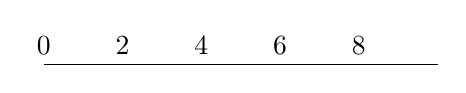
\begin{tikzpicture}
\foreach \n [count = \i] in {0, 2, ..., 8}{
	\node[above] at (\i,0) {\n};
	\draw (\i,0)--($(\i,0)+(1,0)$);
}
\end{tikzpicture}

\subsection{Creating multiple children on a single line}

For a proper loop syntax in forest, see section 3.10 of \href{http://mirrors.ibiblio.org/CTAN/graphics/pgf/contrib/forest/forest-doc.pdf}{forest manual}. A lot of things can be dun just with `repeat` and `append` though:

\begin{forest}
[A,
	repeat=3{ append={ [B] }}
]
\end{forest}

Warning: Putting the tikz foreach cycles inside trees will often not produce the expected results.

\subsection{Defining macros and new commands}

To avoid repetitive text, you can use latex's newcommand, via
\[ \textnormal{ `\textbackslash newcommand\{\textbackslash commandName\}[numberOfParameters1]\{ \dots definition \dots \}', } \]
\noindent Just wrap your repeated text in this with 0 parameters, and re-use it by `\textbackslash commandName\{input1\}\dots\{inputN\}'.



\section{Unresolved issues}

\begin{itemize}
\item Figure out a way to scale pictures with infosets without changing the font size.
\item Pre-defined prettier colors. The current combination is not terrible, but still fairly ugly.
\item Automatically increase the distance between maximizer and minimizer nodes, s.t. they do not need specific treatment and manual adjustment.
	\begin{forest}[,phantom[,pl1][,pl2]]\end{forest} = bad,
	\begin{forest}[,phantom[,pl2][,pl2]]\end{forest} = good.
\item Change anchors of triangle nodes (or do some other magic) s.t. the following picture is vertically aligned.
	\begin{forest}
	delay={for tree={grow=east}}
	[, pl1[, pl2 [, pl1 [, pl2]]]]
	\end{forest} = bad,
	\begin{forest}
	delay={for tree={grow=east, anchor=mid}}
	[, pl1[, pl2 [, pl1 [, pl2]]]]
	\end{forest} = bad,
	\begin{forest}
	[,phantom, s sep+=0.5\nodesize [, pl1] [, pl2] [, pl1] [, pl2] ]
	\begin{pgfonlayer}{bg}
		\draw ($(!1.north)!.5!(!1.south)$)--($(!4.north)!.5!(!4.south)$);
	\end{pgfonlayer}
	\end{forest} = better (but a text inside would still be aligned wrong).	
\end{itemize}

%%%%%%%%%%  Use this example to make sure that your node sizes / l / l sep is correct
%\begin{forest}[
%[,chance[,chance[,chance[,chance[,chance[,chance[,chance[,chance]]]]]]]]
%[,pl1[,pl1[,pl1[,pl1,[,pl1[,pl1[,pl1[,pl1]]]]]]]]
%[,pl2[,pl2[,pl2[,pl2,[,pl2[,pl2[,pl2[,pl2]]]]]]]]
%[0.1,terminal[$\frac 1 2$, terminal[3,terminal [4,terminal [5,terminal [6,terminal [7,terminal [8, terminal]]]]]]]]
%[,pl1[,pl1[,pl2[,chance,[,pl2[,chance[,chance[13,terminal]]]]]]]]
%]
%\node [draw, inner sep = 0em, red, fit=(!1)(!5)] {};
%\node [draw, inner sep = 0em, red, fit=(!11111111)(!31111111)] {};
%\node [draw, inner sep = 0em, red, fit=(!31111111)(!41111111)] {};
%\end{forest}
%%%%%%%%%%%%%%%%%%%%%%%%%%%%%%%%%%%%%%

\newpage
\section{Examples}\label{sec:examples}

\begin{forest}
[,chance
	[,chance
		[,pl1]
		[, phantom [,phantom] [,pl1] ]	
	]
	[,chance
		[,pl1]
		[, phantom [,phantom] [,pl1] ]	
	]
]
\draw (!1)--(!122);
\draw (!2)--(!222);
\node [pl1_cl_infoset, fit=(\corners{!11})(\corners{!21})] {};
\node [pl1_cl_infoset, fit=(\corners{!122})(\corners{!222})] {};
\end{forest}
%
\begin{forest}
[, pl2, l sep-=0.5\nodesize,
	[,chance, edge label={node[midway,sloped,above]{PfA}}
		[,pl1, edge label={node[near start,left]{A}}, [0] ]
		[,pl1, edge label={node[near start,right]{B}}, [1] ]
	]
	[,chance, edge label={node[midway,sloped,above]{PfB}}
		[,pl1, edge label={node[near start,left]{A}}, [1] ]
		[,pl1, edge label={node[near start,right]{B}}, [0] ]
	]
]
\draw [line_infoset, bend right] (!11.south) to (!21.south);
\node[above,yshift=-0.3em] at ($(!121)!.5!(!211)$) {$I_A$};
\draw [line_infoset, bend left] (!12.north) to (!22.north);
\node[above,yshift=0.8\nodesize] at ($(!12)!.5!(!21)$) {$I_B$};
\end{forest}

\begin{figure}[h]
\centering
\begin{forest}
[, chance, l sep-=0.5\nodesize,
	[A,pl1,name=A,
		[0] [1]
	]
	[B,pl1,name=B,
		[1]
		[0]
	]
]
\node [pl1_cl_infoset, fit=(\corners{A})(\corners{B})] {};
\end{forest}
\caption{Caption. Label goes after, or it won't work.}
\label{fig:hist_value_not_unique}
\end{figure}


\end{document}